   \begin{MyInnerSplitBoxLower}{Year 8 and below}
      Find the height of the table.
      \iftoggle{SOLUTION}{%conditional output begin
        \vspace{2.5cm}
      \begin{MySolutionBox}
        If we put the second table on top of the first table on top of the other, the solution becomes obvious!\par
        You can see that the \(130+170\) from the top of the tortoise on the floor to the top of the tortoise on the table is the same as the height of two tables. So the height of one table is \SI{150}{\cm}.
      \end{MySolutionBox}
    }{}%conditional output end
      \tcblower
      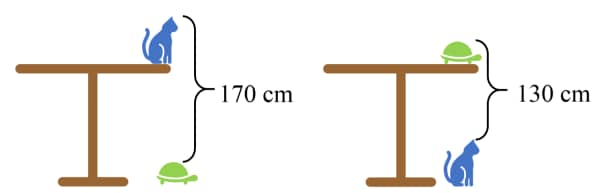
\includegraphics[width=\linewidth]{images/CatTortoiseHeight.jpeg}
      \iftoggle{SOLUTION}{
        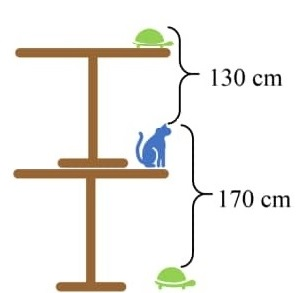
\includegraphics[width=0.5\linewidth]{images/CatTortoiseSoln.jpg}
      }{}
    \end{MyInnerSplitBoxLower}

